\documentclass[12pt]{article}
\usepackage[hmargin={1in},vmargin={1in,1in},foot={.6in}]{geometry}   
\geometry{letterpaper}              
\usepackage{color,graphicx}
\usepackage{setspace}
\usepackage{amsmath}
\usepackage{amssymb}
\usepackage{varioref}
\usepackage{textcomp}
\usepackage{textcomp}
\usepackage{mflogo}
\usepackage{wasysym}
\usepackage[normalem]{ulem}
\usepackage{hyperref}
\usepackage{booktabs}
\usepackage{natbib}

\newcommand{\HRule}{\rule{\linewidth}{0.25mm}}

\usepackage{fancyhdr} % This should be set AFTER setting up the page geometry
\pagestyle{plain} % options: empty , plain , fancy
\lhead{}\chead{}\rhead{}
\renewcommand{\headrulewidth}{.5pt}
\lfoot{}\cfoot{\thepage}\rfoot{}
\newcommand{\txtp}{\textipa}
\renewcommand{\rm}{\textrm}
\newcommand{\sem}[1]{\mbox{$[\![$#1$]\!]$}}
\newcommand{\lam}{$\lambda$}
\newcommand{\lan}{$\langle$}
\newcommand{\ran}{$\rangle$}
\newcommand{\type}[1]{\ensuremath{\left \langle #1 \right \rangle }}

\newcommand{\bex}{\begin{exe}}
	\newcommand{\eex}{\end{exe}}
\newcommand{\bit}{\begin{itemize}}
	\newcommand{\eit}{\end{itemize}}
\newcommand{\ben}{\begin{enumerate}}
	\newcommand{\een}{\end{enumerate}}

\newcommand{\gcs}[1]{\textcolor{blue}{[gcs: #1]}}
\definecolor{Green}{RGB}{10,200,100}
\newcommand{\ndg}[1]{\textcolor{Green}{[ndg: #1]}}

\title{Supporting information: Comparing subjectivity with alternative accounts of adjective order}
%\author{Gregory Scontras, Judith Degen, Noah D.~Goodman}
\date{}

\begin{document}

\maketitle

We have observed the success of adjective subjectivity in predicting ordering preferences for multi-adjective strings. However, we have not compared the predictions of adjective subjectivity with those of alternative proposals. Unfortunately, direct quantitative comparisons prove difficult because the investigations to date have been largely impressionistic. Most authors report their own intuitions or the intuitions of a handful of informants, using a highly constrained set of adjectives and nouns; these data are sufficient for suggesting a potential phenomenon, but we believe insufficient for fully understanding it. The only large-scale empirical studies of ordering preferences are \citet{martin1969}, who limits himself to behavioral measures (i.e., speaker intuitions), and \citet{wulff2003}, who limits herself to corpus measures (i.e., relative frequencies). With respect to ordering preferences, our study marries these two approaches, using both behavioral measures and corpus analyses to arrive at clear estimates of the preferences themselves---showing that there are reliable \emph{quantitative} phenomena to be explained.

There is even less empirical work on the factors that contribute to these ordering preferences. Most authors do not attempt to operationalize their hypotheses, let alone test them in large-scale empirical studies. Once again, \citet{martin1969} stands apart as the sole exception. Of the four different aspects of adjective meaning that he hypothesized would predict ordering preferences, the best-performing measure was adjective ``definiteness;'' it accounts for between 32\% and 55\% of the variance in his preference data.\footnote{\citet{martin1969} tested two sets of twenty adjectives, which he labeled sets A and B. Adjective definiteness accounted for 55\% of the variation in the ordering preferences for set A; for set B, definiteness accounted for 32\% of the variation.} Our study has much wider validity: we use more adjectives, more nouns, and two different operationalizations of subjectivity. Still, understanding the \emph{relative} success of subjectivity in predicting adjective order would aid in understanding its \emph{absolute} success. To that end, here we attempt to operationalize previous accounts so that they may be directly compared with the predictions of subjectivity. We begin at the beginning, with the ``inherentness'' hypothesis from \citet{sweet1898} and \citet{whorf1945}, which we operationalize by recycling the design of an experiment from \citet{martin1969}. Then we look subsectivity, a binary theoretical construct that some linguists have argued underlies ordering preferences \citep[e.g.,][]{truswell2009}. Finally, we try once more to find noun-specific ordering preferences that would support an account based on concept formation, and even attempt to operationalize a concept-formability metric \citep{McNally2004,bouchard2005,svenonius2008}.

\section{The predictive power of inherentness}

Early accounts of adjective ordering proposed that the primary factor derterming order was the ``inherentness'' of the adjectives. We find perhaps the most eloquent assertion of this claim in the following quote from \cite[p.~5]{whorf1945}: 

\begin{quotation}
English adjectives form two main cryptotypes with sub-classes. A group referring to `inherent' qualities---including color, material, physical state (solid, liquid, porous, hard, etc.), provenience, breed, nationality, function, use---has the reactance of being placed nearer the noun than the other group, which we may call one of non-inherent qualities, though it is rather the residuum outside the first group---including adjectives of size, shape, position, evaluation (ethical, esthetic, or economic). These come before the inherent group, e.g. \emph{large red house} (not \emph{red large house}), \emph{steep rocky hill}, \emph{nice smooth floor}.
\end{quotation}

Unfortunately, most authors were content with merely asserting the claim concerning inherentness, not rigorously testing it. Once again, the single outlier is \cite{martin1969}. We ran a version of \citeauthor{martin1969}'s original task, and included a replication of our subjectivity experiment to allow for a direct comparison of the predictions of subjectivity with those of inherentness.

\paragraph{Participants.} We recruited 72 participants through Amazon.com's Mechanical Turk. Participants were compensated for their participation.

\paragraph{Design and methods.} Participants were randomly assigned to one of two conditions: \emph{inherentness} (n=41) or \emph{subjectivity} (n=31). For the inherentness condition, participants rated the ``essentiality'' of adjective-noun object descriptions; they were told that they would be ``asked to decide how essential the adjective is to the meaning of the noun which it modifies, that is, how substantive or inherent the adjective seems in its meaning.'' This language comes from \citeauthor{martin1969}'s original ``substantiveness'' task instructions \citep[Expt.~VII]{martin1969}. Participants indicated their rating using a slider with endpoints labeled ``completely nonessential'' (coded as 0) and ``completely essential'' (coded as 1).

The subjectivity condition was a replication of our original ``subjectivity'' experiment, modified to match the inherentness task. Participants rated the ``subjectivity'' of adjective-noun object descriptions (and not adjectives in isolation; cf.~our \emph{Expt.~1: Subjectivity}); they were told that they would be ``asked to decide how subjective the adjective seems in its meaning.'' Participants indicated their rating using a slider with endpoints labeled ``completely objective'' (coded as 0) and ``completely subjective'' (coded as 1).

Participants completed a total of 26 trials, one for each of the adjectives in Table 1; nouns were chosen at random from the list in Table 1. All 72 participants indicated that they were native speakers of English; we analyze their data below.

\paragraph{Results.} We averaged the inherentness and subjectivity scores for each adjective. Fig.~\ref{fig:inherentness} plots mean inherentness (\emph{left}) and subjectivity (\emph{right}) scores against the inferred distance naturanless scores from \textit{Expt.~1: Ordering preferences}. As Fig.~\ref{fig:inherentness} demonstrates, inherentness does little to predict ordering preferences, accounting for 0.0\% of the variance in the naturalness ratings ($r^2${=}0.00, 95\% CI [0.00,  0.02]). However, we have replicated the success of adjective subjectivity, which accounts for 75\% of the variation in the naturalness ratings ($r^2${=}0.75, 95\% CI [0.53,  0.84]).

\renewcommand\thefigure{S.\arabic{figure}}
\begin{figure}
	\centering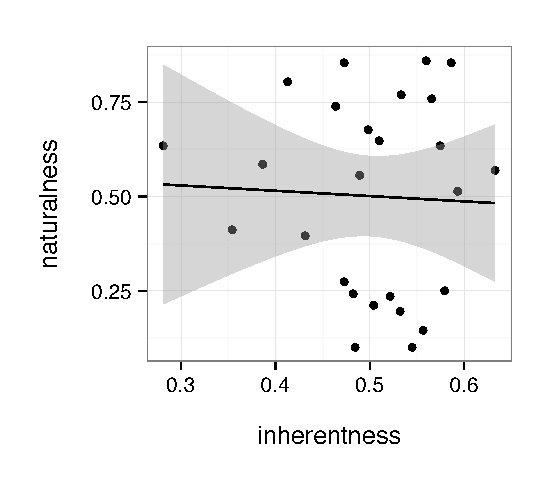
\includegraphics[width=3in]{plots/expt1-inherentness-naturalness.eps}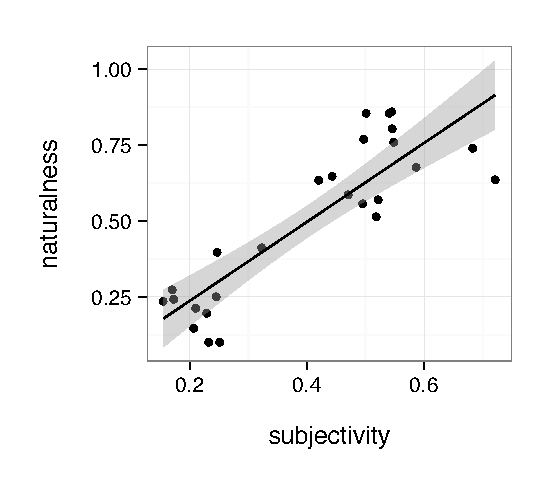
\includegraphics[width=3in]{plots/expt1-subjectivity2-naturalness.eps}
	\caption{Mean naturalness ratings plotted against mean inherentness (\emph{left}) and subjectivity (\emph{right}) scores for each of the 26 adjectives tested.}\label{fig:inherentness}
\end{figure}

\paragraph{Discussion.} Using a modified version of \citeauthor{martin1969}'s (\citeyear{martin1969}) task measuring adjective inherentness, we failed to find \emph{any} correlation between inherentness and ordering preferences for our set of 26 adjectives. Indeed, our findings match \citeauthor{martin1969}'s own: he documented that inherentness accounted for between 14\% and 3\% of the variation in the ordering preferences that he measured for 40 adjectives. We also measured adjective subjectivity, which allows for a direct comparison of the two predictors: whereas inherentness accounted for no variation, subjectivity accounted for 75\% of the variation in our ordering preferences. Despite the many claims to its success in the literature \citep[e.g.,][]{sweet1898,whorf1945,kemmerer2000}, adjective inherentness does little (or nothing) to explain the observed regularities in adjective order. However, subjectivity continues to predict ordering preferences.



\section{Subjectivity vs.~subsectivity}

Next, we turn to a more abstract but no less popular factor meant to account for ordering preferences: the logical distinction between intersectivity and subsectivity. Semanticists argue that adjectives split on the basis of how they modify the nouns with which they compose \citep[for discussion, see][]{kamppartee1995}. Some adjectives are \emph{intersective}: the outcome of their modification is the intersection of the nominal denotation with the adjectival denotation, as in the following example, where \emph{carnivorous mammal} describes those things that hold the property of being carnivorous and of being a mammal.

\begin{align*} 
\sem{carnivorous} &= \{x : carnivorous(x)\}\\
\sem{mammal} &= \{x : mammal(x)\}\\
\sem{carnivorous mammal} &= \{x : carnivorous(x)\ \&\ mammal(x)\}\\
& =\sem{carnivorous} \cap \sem{mammal}
\end{align*}

\noindent Other adjectives are \emph{subsective}: rather than intersecting with a nominal denotation, the outcome of subsective modification is a subset of the nominal denotation, which is used to determine the comparison class for the adjective. Subsective adjectives depend on the nominal with which they compose to fix their meaning. Take \emph{skillful}: a skillful surgeon is not necessarily a skillful violinist, but a skillful surgeon is necessarily a surgeon:

\begin{align*} 
\sem{skillful surgeon} & \subseteq \sem{surgeon}
\end{align*}

\noindent Finally, there are those adjectives that are neither clearly intersective nor clearly subsective. The most obvious cases are so-called \emph{privative} adjectives like \emph{fake}, which require that the outcome of modification is a proper complement of the nominal denotation: a fake gun is not a gun.  More generally, these non-intersective, non-subsective adjectives preclude the inference that the things described hold the property named by the noun:

\begin{align*} 
\sem{fake gun} & \nsubseteq \sem{gun}\\
\sem{former senator} & \nsubseteq \sem{senator}
\end{align*}

What matters for present purposes is that some authors assume that the means of modification determines adjective order, such that intersective adjectives occur closer to the noun than subsective adjectives. We find the clearest statement of this claim in \cite{truswell2009}, who assumes that hierarchical dominance leads to linear precedence:

\begin{quotation}
\noindent\ben
	\item Subsective adjectives dominate intersective adjectives. \item Modal [(i.e., non-subsective)] adjectives are freely ordered with respect to subsective and intersective adjectives, although they tend to dominate both classes.
	\een
\end{quotation}

\noindent According to \citeauthor{truswell2009}, intersective adjectives occur closest to the modified noun, subsective adjectives occur farther than intersective adjectives, and non-subsective adjectives are freely ordered, despite their tendency to occur farthest of all. 

There are two reasons why we do not consider subsectivity to be a true competitor to the subjectivity hypothesis. First, the intersective--subsective distinction is not a behavioral measure, nor even a human concept; the distinction is theoretical, and it takes consultation with a trained linguist to fix the status of a given adjective. Compare this with subjectivity, where we have seen the success of two behavioral measures with naive participants. Even more problematic is the fact that the intersective--subsective distinction is a binary one, but we have seen systematic graded behavior in the ordering of adjectives.

Still, we attempted to compare the predictions of the two proposals. To do so, we coded our adjectives as either \emph{subsective}, \emph{intersective}, or \emph{other} using \citeauthor{truswell2009}'s classifications: shape, color, nationality, and material adjectives were coded as \emph{intersective}; all other adjectives were coded as \emph{subsective}, except for the non-intersective class ``X'' adjectives from Expt.~2, which we coded as \emph{other}.

The first thing to note is that the two predictors (i.e., subjectivity and subsectivity) are extremely highly correlated (Expt.~1: $r^2${=}0.89, 95\% CI [0.74,  0.94]; Expt.~2: $r^2${=}0.52, 95\% CI [0.35,  0.65]). This correlation should come as no surprise, given that the intersective--subsective distinction hangs on the context sensitivity of the adjective: intersective adjectives have fixed interpretations (i.e., they are maximally objective), while the interpretation of subsective adjectives varies with the modified noun. Given this high correlation and the observed success of subjectivity in predicting ordering preferences, we expect subsectivity to do well in predicting ordering preferences. However, the binary nature of the subsectivity predictor cannot account for the variation \emph{within} the classes of subsective and intersective adjectives. 

\renewcommand\thefigure{S.\arabic{figure}}
\begin{figure}
	\centering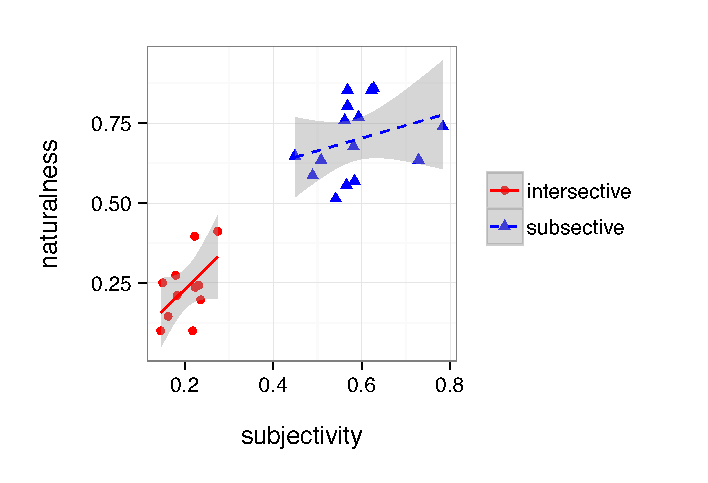
\includegraphics[width=4.5in]{plots/expt1-subjectivity-subsectivity.eps}\\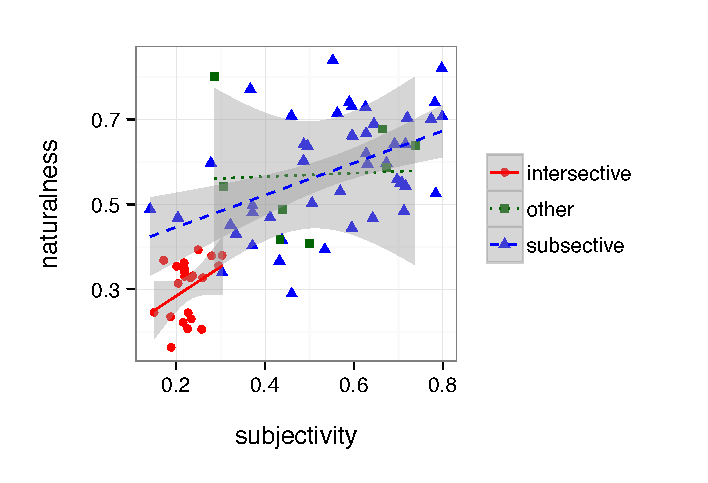
\includegraphics[width=4.5in]{plots/expt3-subjectivity-subsectivity.eps}
	\caption{Mean naturalness ratings plotted against mean subjectivity scores grouped by subsectivity for the original set of 26 adjectives tested in Expt.~1 (\emph{top}) and the expanded set of 78 adjectives tested in Expt.~2 (\emph{bottom}).}\label{fig:subsectivity}
\end{figure}

Fig.~\ref{fig:subsectivity} plots adjective subjectivity scores against naturalness ratings from Expt.~1 (\emph{top}) and Expt.~2 (\emph{bottom}), grouping adjectives by subsectivity class. To evaluate the role of subjectivity \emph{over an above subsectivity} in predicting ordering preferences, we performed a nested model comparison. The models we compared predicted naturalness ratings by \textsc{subsectivity} only, or by \textsc{subsectivity} and \textsc{subjectivity}. The model comparison revealed that subjectivity does explain additional variance in ording preferences beyond the intersective--subsective distinction (Expt.~1: $F(1,2337)=25.28, p<0.001$; Expt.~2: $F(1,23786)=361.78, p<0.001$): as Fig.~\ref{fig:subsectivity} shows, even within the subsectivity classes, subjectivity continues to predict ordering preferences. Thus, we continue to find support for the subjectivity hypothesis.


\section{Testing compositional accounts}

Compositional accounts of ordering preferences hold that the fundamental factor in predicting adjective ordering is whether or not an adjective is used to form a complex concept/subkind description: first you form the concept, then you modify it with additional adjectives \citep{McNally2004,svenonius2008}.\footnote{\cite{bouchard2005} makes a similar claim, namely that the formation of complex concepts can override adjective ordering preferences.} 
This would imply that an interaction between the noun and a modifying adjective---whether they combine to form a complex concept---should have a large influence on adjective ordering. 
Indeed, a more general hypothesis is that \emph{some} interaction between a noun and adjective will influence how closely the adjective is placed to that noun. This interaction could be caused by concept-formation, differential subjectivity, or other factors. We tested for such an interaction in Expt.~1 and in Expt.~2, and found that noun-specific naturalness did not explain any variance in ordering preference above and beyond adjective-level naturalness. %Looking in more detail, there were two adjective-noun pairs in our data with trends in the predicted direction: the naturalness ratings for \emph{hard} and \emph{soft} suggested a preference to occur closer to the noun \emph{cheese}. (Plausibly because hard and soft cheeses are natural kinds.) While these adjective-noun interactions do not survive correction for multiple comparisons in our statistical analysis, they do indicate that a different set of materials might reveal by-noun effects on ordering preference. 
Here we follow up on this result, first with a new set of materials that were chosen to maximize the probability of noun effects, and then with our attempt at operationalizing a concept-formability metric.

\subsection{In search of noun effects}

This experiment was a direct replication of \emph{Expt.~1.1 Ordering preferences}, using a different set of nouns. We aimed to choose nouns that formed idiomatic, complex concepts with our set of 26 adjectives. Complex concepts tend to be described using the two-word name, yielding more occurrences of this bigram than would be expected from the unigram frequencies of the noun and adjective. This provided a way to extract candidate complex concepts from corpora.

 %with the given adjectives and therefore yield effects on ordering preferences.

\paragraph{Participants.}

We recruited 50 participants through Amazon.com's Mechanical Turk crowd-sourcing service. Participants were compensated for their participation.

\paragraph{Design and methods.}

The design was identical to our original naturalness ratings experiments: participants were asked to indicate which of two object descriptions sounded more natural, using a sliding scale. Each description featured a noun modified by two adjectives; description pairs contained the same words with the relative adjective order reversed (e.g., ``the big blue thing'' vs.~``the blue big thing''). Adjectives were chosen at random from the set in Table 1. The nouns were a smaller set of five (compared to the original ten). Nouns were chosen to maximize the probability of detecting noun-specific effects on adjective ordering preferences. In particular, we expected that nouns that are likely to form complex concepts should be 
highly collocational with that adjective. We thus searched for nouns that occur in particular adjective-noun phrases more frequently than predicted by the individual noun and adjective probabilities; in other words, nouns whose adjective-noun combinations were under-predicted by their individual word probabilities. 

To find these nouns, we estimated the probability $p(A)$ of each adjective from our set of 26 by computing its relative frequency in an adjective-noun sequence in the BNC. We then computed the relative frequency of each noun $p(N)$ occurring in an adjective-noun sequence. Finally, we estimated the predicted joint probability of each adjective-noun combination by taking the product of each individual probability estimate: $\hat{p}(A,N) = p(A)\cdot p(N)$. Comparing  $\hat{p}(A,N)$ to the empirically estimated $p(A,N)$ establishes which adjective-noun combinations are under-predicted---more collocational---and thus likely to name complex concepts. We then restricted nouns to those 50 that maximize the observed range of under-predictedness while simultaneously requiring that each noun be attested to occur with at least 11 of the 26 adjectives; from these 50 nouns, we selected the following four: \emph{apple, cheese, eyes, hair}.\footnote{We restricted to a small subset of the 50 target nouns in order to maximize statistical power to identify noun effects on ordering.} (Recall that \emph{cheese} occurred in our original materials, where it suggested possible by-noun effects with the adjectives \emph{hard} and \emph{soft}.) To these four nouns we added a fifth: \emph{thing}.
While \emph{thing} did not occur in the top 50, it did occur naturalistically with the most adjectives (23) out of the set of 26, thus allowing it to serve as a filler for the various object descriptions. The selected nouns, together with the number of adjectives they occur with, their range of ratios of empirical to predicted joint probabilities, and their minimum / maximum ratios, are shown in Table \ref{tab:nouns}.

\renewcommand\thetable{S.\arabic{table}}
\begin{table}
\centering
\begin{tabular}{l c c c c}
\toprule
Noun & \# of adjectives & range of ratios & minimum ratio & maximum ratio\\
\midrule
thing & 23 & 10.4 & 0.1 & 10.5 \\
eyes & 18 & 120.6 & 0.12 & 120.7 \\
hair & 15 & 82.9 & 0.03 & 83.0 \\
cheese & 13 & 114.0 & 0.4 & 114.4 \\
apple & 11 & 674.0 & 1.1 & 675.1 \\
\bottomrule
\end{tabular}
\caption{For each chosen noun, the number of adjectives (out of 26) that it occurs with; and for each adjective $A$ that the noun occurs with, the range of ratios $p(A,N) / \hat{p}(A,N)$ (empirical to predicted probability of occurrence); the minimum ratio; and the maximum ratio.}
\label{tab:nouns}
\end{table}




\paragraph{Results.}

To evaluate the role of specific noun information in determining ordering preferences, we performed the same nested linear model comparison from our original naturalness ratings experiment. The models we compared predicted naturalness ratings either by \textsc{adjective} (i.e., the adjective farthest from the noun) only, or by \textsc{adjective} together with its interaction with \textsc{noun} (i.e., the modified noun).
The model comparison revealed that noun-specific ratings did not explain any additional variance in ordering preference beyond adjective-level ratings ($F(1,104) = 1.10, p < 0.30$).  Thus, we again fail to find evidence of noun-specific effects on ordering preferences in our new materials. 


%\subsection{Subjectivity}
%
%We next set out to replicate the finding that subjectivity predicts adjective ordering preferences in our new materials.
%
%\paragraph{Participants.}
%
%We recruited 40 participants through Amazon.com's Mechanical Turk crowd-sourcing service. Participants were compensated for their participation.
%
%\paragraph{Design and methods.}
%
%This experiment was a direct replication of our original faultless disagreement subjectivity experiment (Experiment 3), using the new set of nouns from the previous experiment.

%\paragraph{Predicting adjective order.}

Given the lack of noun effects on ordering preferences, we should continue to find that adjective subjectivity predicts ordering preferences. Indeed, it does: adjective subjectivity scores (obtained in \emph{Expt 1.2 Subjectivity}) account for  85\% of the variance in the new naturalness ratings ($r^2${=}0.85, 95\% CI [0.64,  0.93]; Fig.~\ref{fig:subjectivity}). 
%Faultless disagreement scores account for  84\% of the variance in the new naturalness ratings ($r^2$ 0.84, 95\% CI [0.64,  0.91]; Fig.~\ref{fig:faultless}). 
As with our original materials, more subjective adjectives are preferred farther from the noun.


\renewcommand\thefigure{S.\arabic{figure}}
\begin{figure}
	\centering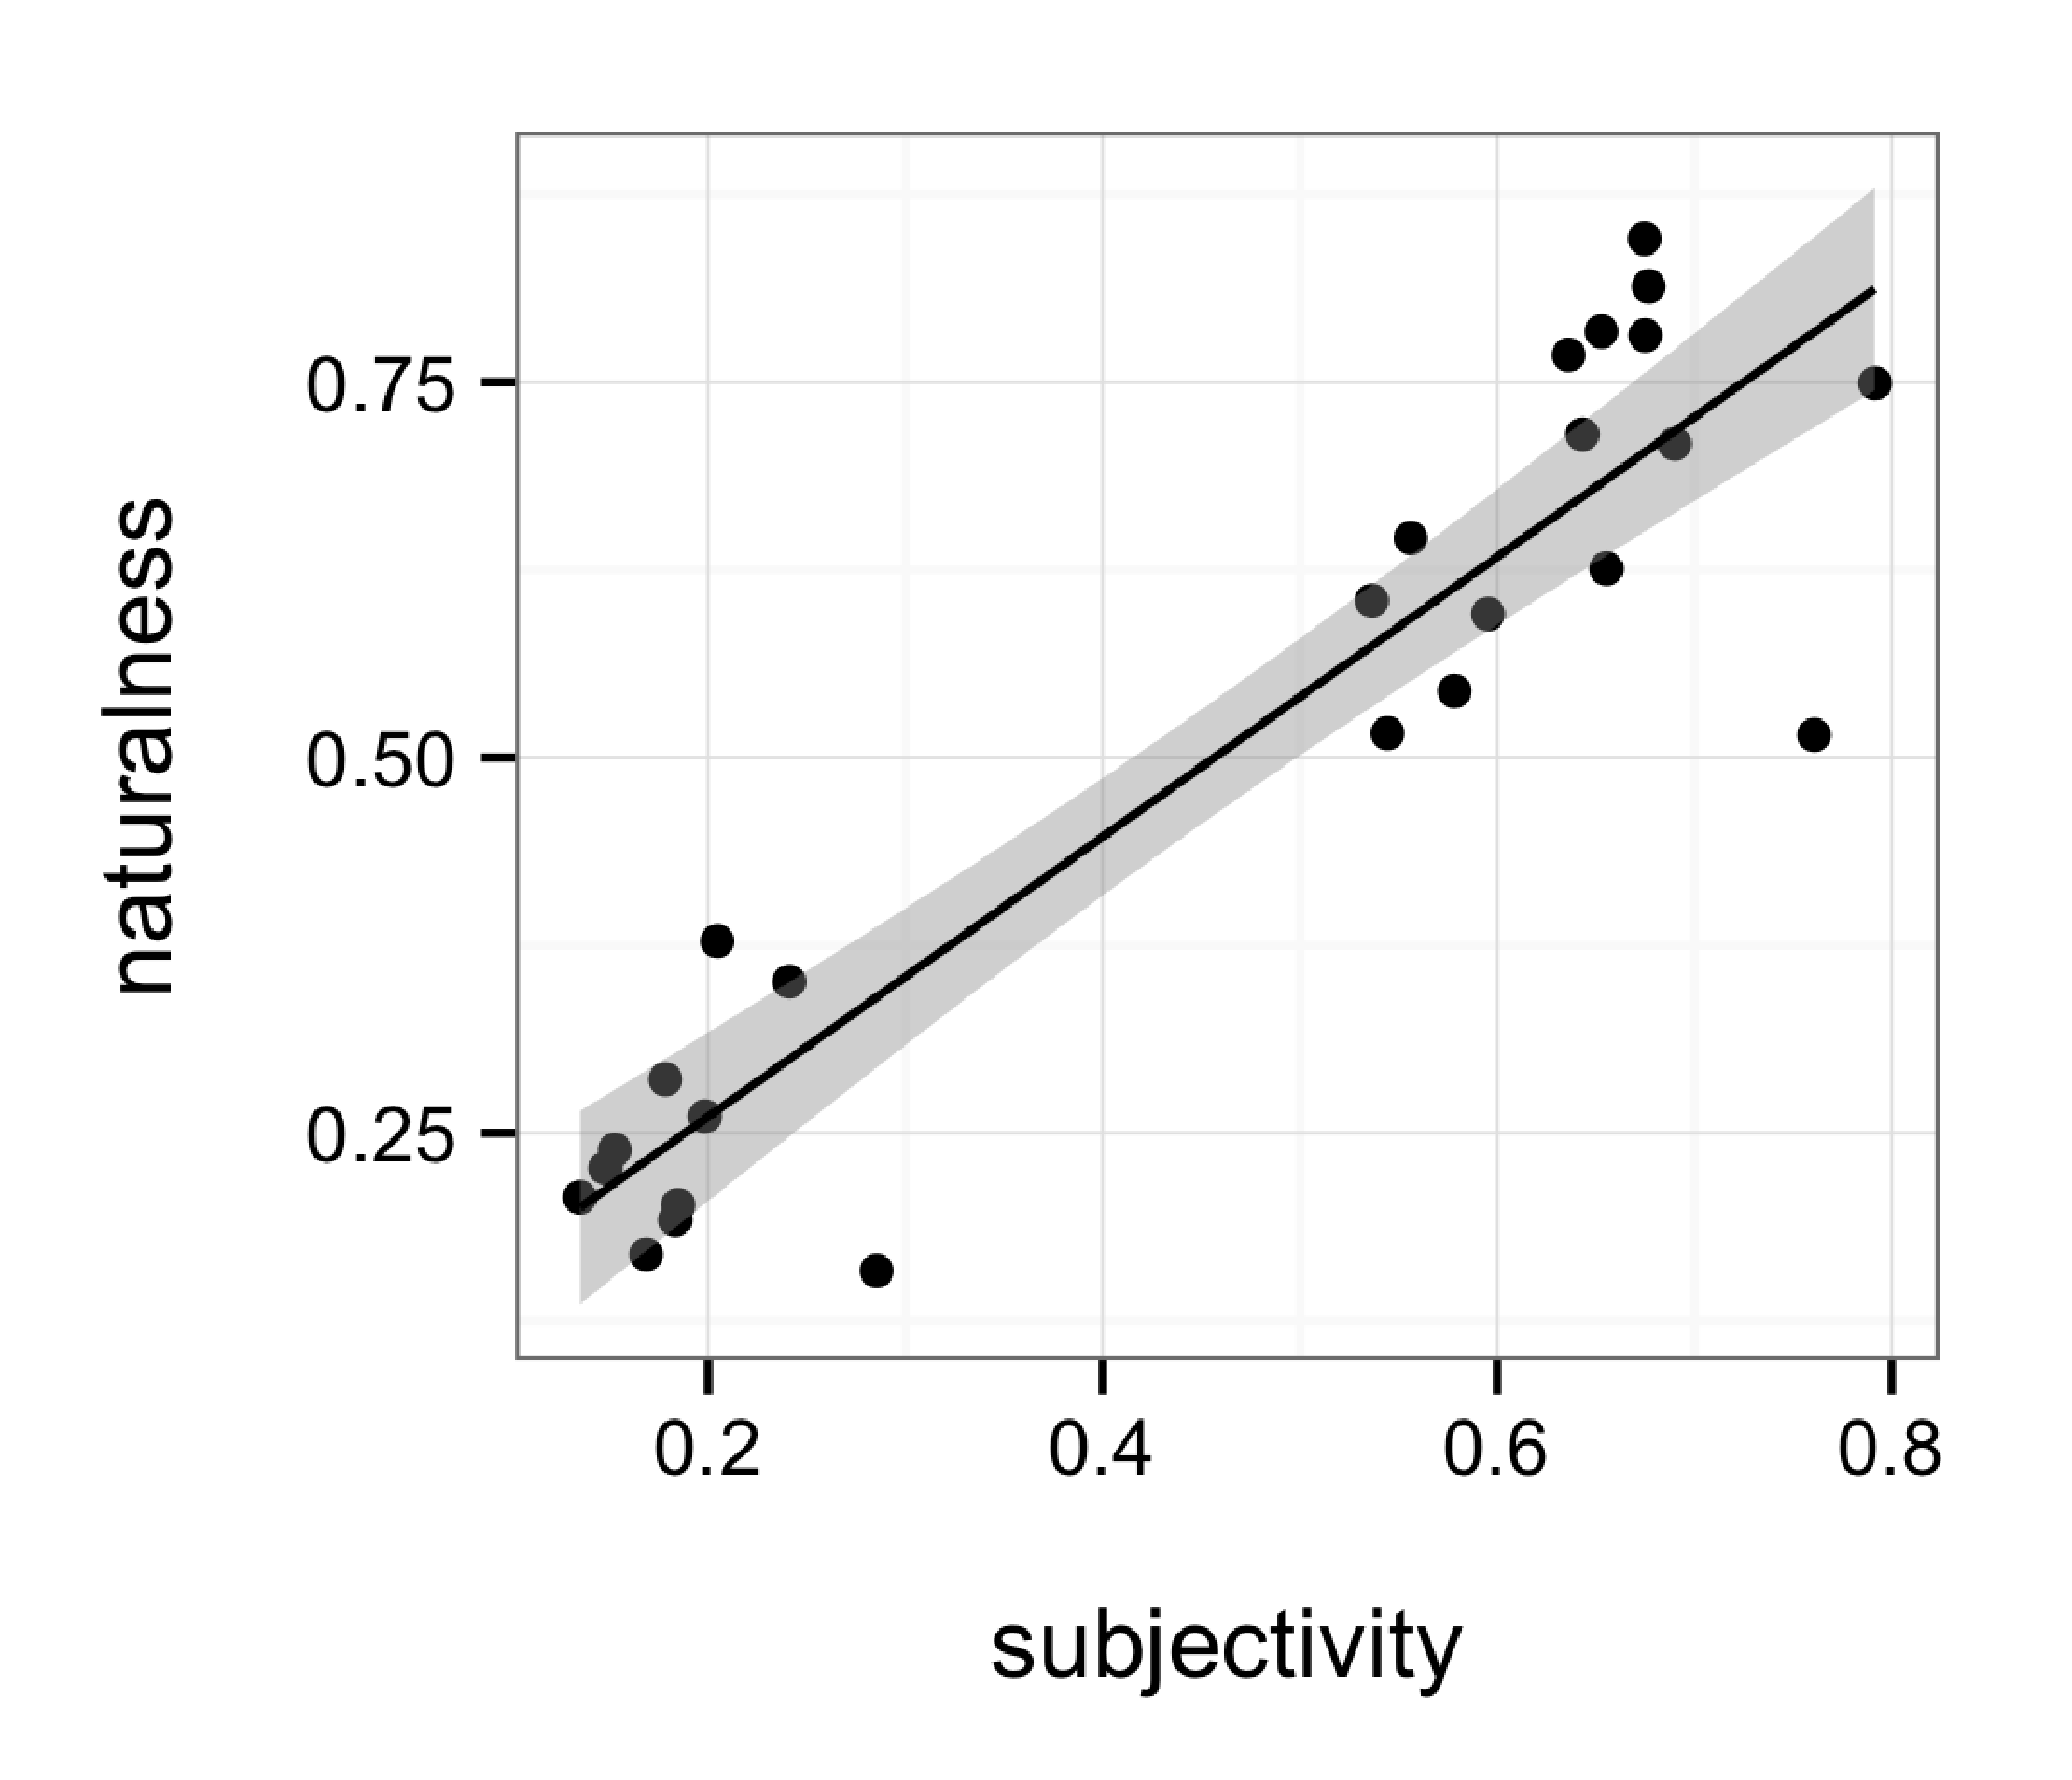
\includegraphics[width=3.5in]{plots/naturalness-subjectivity-new-nouns.eps}
	\caption{Mean naturalness ratings plotted against mean subjectivity scores for each of the 26 adjectives tested in the new order preference experiment.}\label{fig:subjectivity}
\end{figure}

\paragraph{Discussion.} Using nouns chosen to maximize the probability of complex concepts formed with our 26 adjectives, we failed to find evidence that adjective ordering preferences depend on the modified noun. We do continue to find that subjectivity predicts ordering preferences. Thus, we failed to find evidence in support of compositional accounts of ordering preferences, which hold that the most important factor in determining order is whether or not an adjective forms a complex concept with the noun it modifies. 
It remains possible that noun-effects (and hence effects of concept composition) would be found with a different set of adjectives. 
However, this already suggests that the effect of modified nouns explains only a small part of the overall story of adjective order; subjectivity seems to do better.



\subsection{Operationalizing concept-formability}

Failing to find support for the most general prediction of the compositional account, namely an effect of nouns on ordering preferences, we tried a more targeted approach: operationalizing a concept-formability metric, and testing its predictions on the adjective ordering preferences that we measured in \emph{Expt.~1: Ordering preferences}. As with the studies in our paper, the work lies in operationalizing an abstract notion like whether or not an adjective tends to form a complex concept. The literature on the topic presupposes that intuitions about concept formability are systematic and generalizable \citep{McNally2004,svenonius2008}; the closest we found in these papers to a proposal for an empirical measure of this factor is the following distinction.

According to \citeauthor{McNally2004}, the key issue is one of entailment. When an adjective modifies a noun intersectively, the objects described hold both the property named by the noun and the property named by the adjective: a ``male architect'' is both male and an architect \citep[p.~179, ex.~2]{McNally2004}. When an adjective and a noun combine to form a complex concept (i.e., a subkind description), the objects described hold the property named by the noun, but not necessarily the property named by the adjective; the modification is (ostensibly) subsective. The authors give the Catalan example \emph{arquitecte t\`{e}cnic} ``technical architect,'' which names a kind of architect but not necessarily technical things (\citealp[p.~179, ex.~1]{McNally2004}; cf.~the discussion of \emph{wild rice} in \citealp{svenonius2008}).\footnote{This distinction should ring familiar from the discussion of intersective vs.~subsective modification above.} 
Using our original set of materials, we tested whether the objects named by an adjective-noun description hold 1) the property named by the adjective, and 2) the property named by the noun.

%Suppose the fundamental factor in predicting adjective ordering is whether an adjective is used to form a complex concept/subkind description or not.

%We find this hypothesis intriguing---perhaps concept-formability indeed determines ordering preferences (and therefore correlates with subjectivity)? The semantic analysis given by these authors to adjectives that form complex concepts requires them to compose first with nouns, before run-of-the-mill intersective adjectives; thus, the fundamental factor in predicting adjective ordering ought to be whether an adjective forms a complex concept. Does concept-formability predict ordering preferences?


\paragraph{Participants.} We recruited 40 participants through Amazon.com's Mechanical Turk.  Participants were compensated for their participation.

\paragraph{Design and methods.} Participants were presented with 26 adjective-noun object descriptions. They were instructed to ``consider the things that might be described'' as \texttt{adjective-noun} (e.g., ``round desks''), then rate how likely it is that the things described 1) hold the \texttt{adjective} property (e.g., ``Are those things round?''), and 2) hold the \texttt{noun} property (e.g., ``Are those things desks?''). Participants indicated their probability ratings using sliders with endpoints labeled with ``definitely not'' (coded as 0) and ``definitely'' (coded as 1).\footnote{The full experiment is \href{http://web.stanford.edu/~scontras/adjective_ordering/experiments/9-concept-formability/concept-formability.html}{viewable online here}.} All 40 participants indicated that their native language was English; we report their results below.

\paragraph{Results.} We averaged probability scores for each adjective. Fig.~\ref{fig:concept} plots the adjective (\emph{left}) and noun (\emph{right}) scores against the naturalness ratings from \emph{Expt.~1: Ordering preferences}. According to the predictions of the compositional account, lower adjective probability should lead to higher naturalness: as the property named by an adjective is less likely to apply straightforwardly to the objects named, the probability that the adjective forms a complex concept with the noun it modifies increases. While we do observe this trend in Fig.~\ref{fig:concept}, we also see that adjective probability scores predict just 8\% of the variance in our preference data (r$^{2}=0.08$; 95\% CI [0.00,  0.33]). %The noun ratings do better, explaining 36\% of the variance (r$^{2}=0.36$; 95\% CI [0.07,  0.62]).


\renewcommand\thefigure{S.\arabic{figure}}
\begin{figure}
	\centering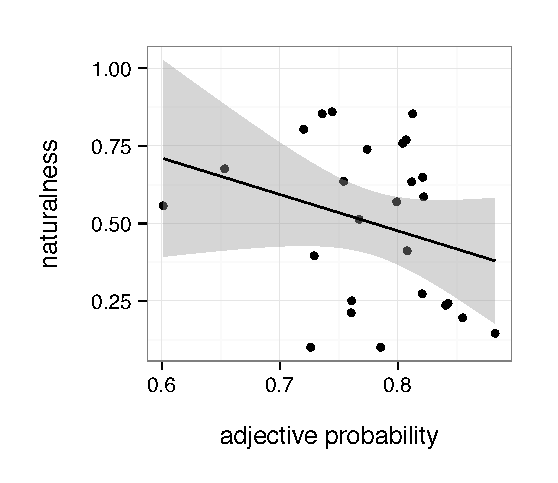
\includegraphics[width=3.5in]{plots/naturalness-concept-adjective.eps}%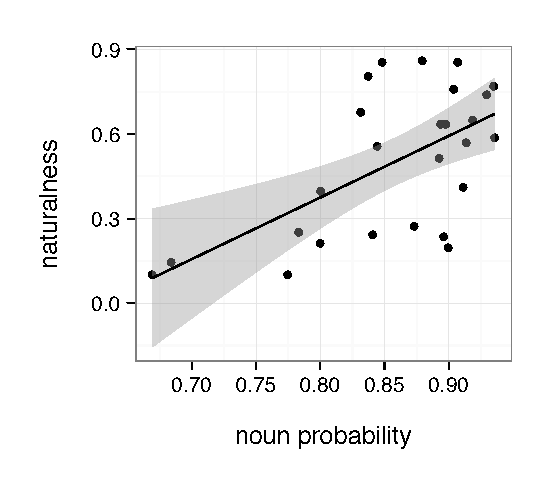
\includegraphics[width=3in]{plots/naturalness-concept-noun.eps}
	\caption{Mean naturalness ratings plotted against mean adjective probability (i.e., concept-formability) scores for each of the 26 adjectives tested.}\label{fig:concept}
\end{figure}

\paragraph{Discussion.} Recall that at its worst, subjectivity predicts 70\% of the variance in our preference data. 
While it is quite possible that concept-formability plays an important role for some cases (such as \emph{arquitecte t\`{e}cnic}), we did not find evidence that it was critical to ordering preferences in our broad set of items. 

\section{Conclusion}

We have compared the subjectivity hypothesis with the predictions of three alternative accounts of adjective order: inherentness, subsectivity, and concept-formability. Our results demonstrate the robust replicability of the success of subjectivity in predicting adjective order. The results also demonstrate that the alternative accounts we considered add little to our understanding of ordering preferences: everywhere we looked, subjectivity continued to predict ordering preferences. This exploration has led us to better appreciate the intuitive appeal of the subjectivity hypothesis, which targets an easily-accessed, stable psychological construct: adjective subjectivity.





\bibliographystyle{chicago} 
\bibliography{adjectives}


\end{document}










Compositional (i.e., semantic) accounts of ordering preferences hold that the fundamental factor in predicting adjective ordering is whether or not an adjective is used to form a complex concept/subkind description: first you form the concept, then you modify it with additional adjectives (McNally and Boleda, 2004; Svenonius, 2008).\footnote{Bouchard 2005 makes a similar claim, namely that the formation of complex concepts can override adjective ordering preferences.} 
This would imply that an interaction between the noun and a modifying adjective---whether they combine to form a complex concept---should have a large influence on adjective ordering. 
Indeed, a more general hypothesis is that \emph{some} interaction between a noun and adjective will influence how closely the adjective is placed to that noun. This interaction could be caused by concept-formation, differential subjectivity, or other factors. We tested for such an interaction in our original naturalness ratings and found that noun-specific naturalness did not explain any variance in ordering preference above and beyond adjective-level naturalness. However, there were two adjective-noun pairs in our data with trends in the predicted direction: the naturalness ratings for \emph{hard} and \emph{soft} suggested a preference to occur closer to the noun \emph{cheese}. (Plausibly because hard and soft cheeses are complex concepts.) While these adjective-noun interactions do not survive correction for multiple comparisons in our statistical analysis, they do indicate that a different set of materials might reveal by-noun effects on ordering preference. To follow up on this possibility, we re-ran our order preference and subjectivity experiments with a new set of materials that were chosen to maximize the probability of noun effects.


\section*{Experiment S1: Ordering preferences}

This experiment was a direct replication of our original naturalness ratings experiment (Experiment 1), using a different set of nouns. We chose nouns that we expected to form complex concepts with the given adjectives and therefore yield effects on ordering preferences.

\paragraph{Participants.}

We recruited 50 participants through Amazon.com's Mechanical Turk crowd-sourcing service. Participants were compensated for their participation.

\paragraph{Design and methods.}

The design was identical to our original naturalness ratings experiment: participants were asked to indicate which of two object descriptions sounded more natural, using a sliding scale. Each description featured a noun modified by two adjectives; description pairs contained the same words with the relative adjective order reversed (e.g., ``the big blue thing'' vs.~``the blue big thing''). Adjectives were chosen at random from the original set of 26. The nouns were a smaller set of five (compared to the original ten). Nouns were chosen to maximize the probability of detecting noun-specific effects on adjective ordering preferences. In particular, we expected that nouns that are likely to form complex concepts should be 
highly collocational with that adjective. We thus searched for nouns that occur in particular adjective-noun phrases more frequently than predicted by the individual noun and adjective probabilities; in other words, nouns whose adjective-noun combinations were under-predicted by their individual word probabilities. 

To find these nouns, we estimated the probability $p(A)$ of each adjective from our set of 26 by computing its relative frequency in an adjective-noun sequence in the BNC. We then computed the relative frequency of each noun $p(N)$ occurring in an adjective-noun sequence. Finally, we estimated the predicted joint probability of each adjective-noun combination by taking the product of each individual probability estimate: $\hat{p}(A,N) = p(A)\cdot p(N)$. Comparing  $\hat{p}(A,N)$ to the empirically estimated $p(A,N)$ establishes which adjective-noun combinations are under-predicted---more collocational---and thus likely to name complex concepts. We then restricted nouns to those 50 that maximize the observed range of under-predictedness while simultaneously requiring that each noun be attested to occur with at least 11 of the 26 adjectives; from these 50 nouns, we selected the following four: \emph{apple, cheese, eyes, hair}. (Recall that \emph{cheese} occurred in our original materials, where it suggested possible by-noun effects with the adjectives \emph{hard} and \emph{soft}.) To these four nouns we added a fifth: \emph{thing}.
While \emph{thing} did not occur in the top 50, it did occur naturalistically with the most adjectives (23) out of the set of 26, thus allowing it to serve as a filler for the various object descriptions. The selected nouns, together with the number of adjectives they occur with, their range of ratios of empirical to predicted joint probabilities, and their minimum / maximum ratios, are shown in Table \ref{tab:nouns}.

\renewcommand\thetable{S.\arabic{table}}
\begin{table}
	\centering
	\begin{tabular}{l c c c c}
		\toprule
		Noun & \# of adjectives & range of ratios & minimum ratio & maximum ratio\\
		\midrule
		thing & 23 & 10.4 & 0.1 & 10.5 \\
		eyes & 18 & 120.6 & 0.12 & 120.7 \\
		hair & 15 & 82.9 & 0.03 & 83.0 \\
		cheese & 13 & 114.0 & 0.4 & 114.4 \\
		apple & 11 & 674.0 & 1.1 & 675.1 \\
		\bottomrule
	\end{tabular}
	\caption{For each chosen noun, the number of adjectives (out of 26) that it occurs with; and for each adjective $A$ that the noun occurs with, the range of ratios $p(A,N) / \hat{p}(A,N)$ (empirical to predicted probability of occurrence); the minimum ratio; and the maximum ratio.}
	\label{tab:nouns}
\end{table}




\paragraph{Results.}

To evaluate the role of specific noun information in determining ordering preferences, we performed the same nested linear model comparison from our original naturalness ratings experiment. The models we compared predicted naturalness ratings either by \textsc{adjective} (i.e., the adjective farthest from the noun) only, or by \textsc{adjective} together with its interaction with \textsc{noun} (i.e., the modified noun).
The model comparison revealed that noun-specific ratings did not explain any additional variance in ordering preference beyond adjective-level ratings ($F(1,225) = 0.93, p < 0.75$).  Thus, we again fail to find evidence of noun-specific effects on ordering preferences, this time in our new materials. 

\section*{Experiment S2: Subjectivity}

We next set out to replicate the finding that subjectivity predicts adjective ordering preferences in our new materials.

\paragraph{Participants.}

We recruited 40 participants through Amazon.com's Mechanical Turk crowd-sourcing service. Participants were compensated for their participation.

\paragraph{Design and methods.}

This experiment was a direct replication of our original faultless disagreement subjectivity experiment (Experiment 3), using the new set of nouns from the previous experiment.

\paragraph{Results.}

To evaluate the power of subjectivity in predicting adjective ordering preferences, we compared our new adjective subjectivity scores to the naturalness ratings collected in the previous experiment. 
Faultless disagreement scores account for  84\% of the variance in the new naturalness ratings ($r^2$ 0.84, 95\% CI [0.64,  0.91]; Fig.~\ref{fig:faultless}). 
As with our original materials, more subjective adjectives are preferred farther from the noun; subjectivity again predicts adjective ordering preferences.


\renewcommand\thefigure{S.\arabic{figure}}
\begin{figure}
	\centering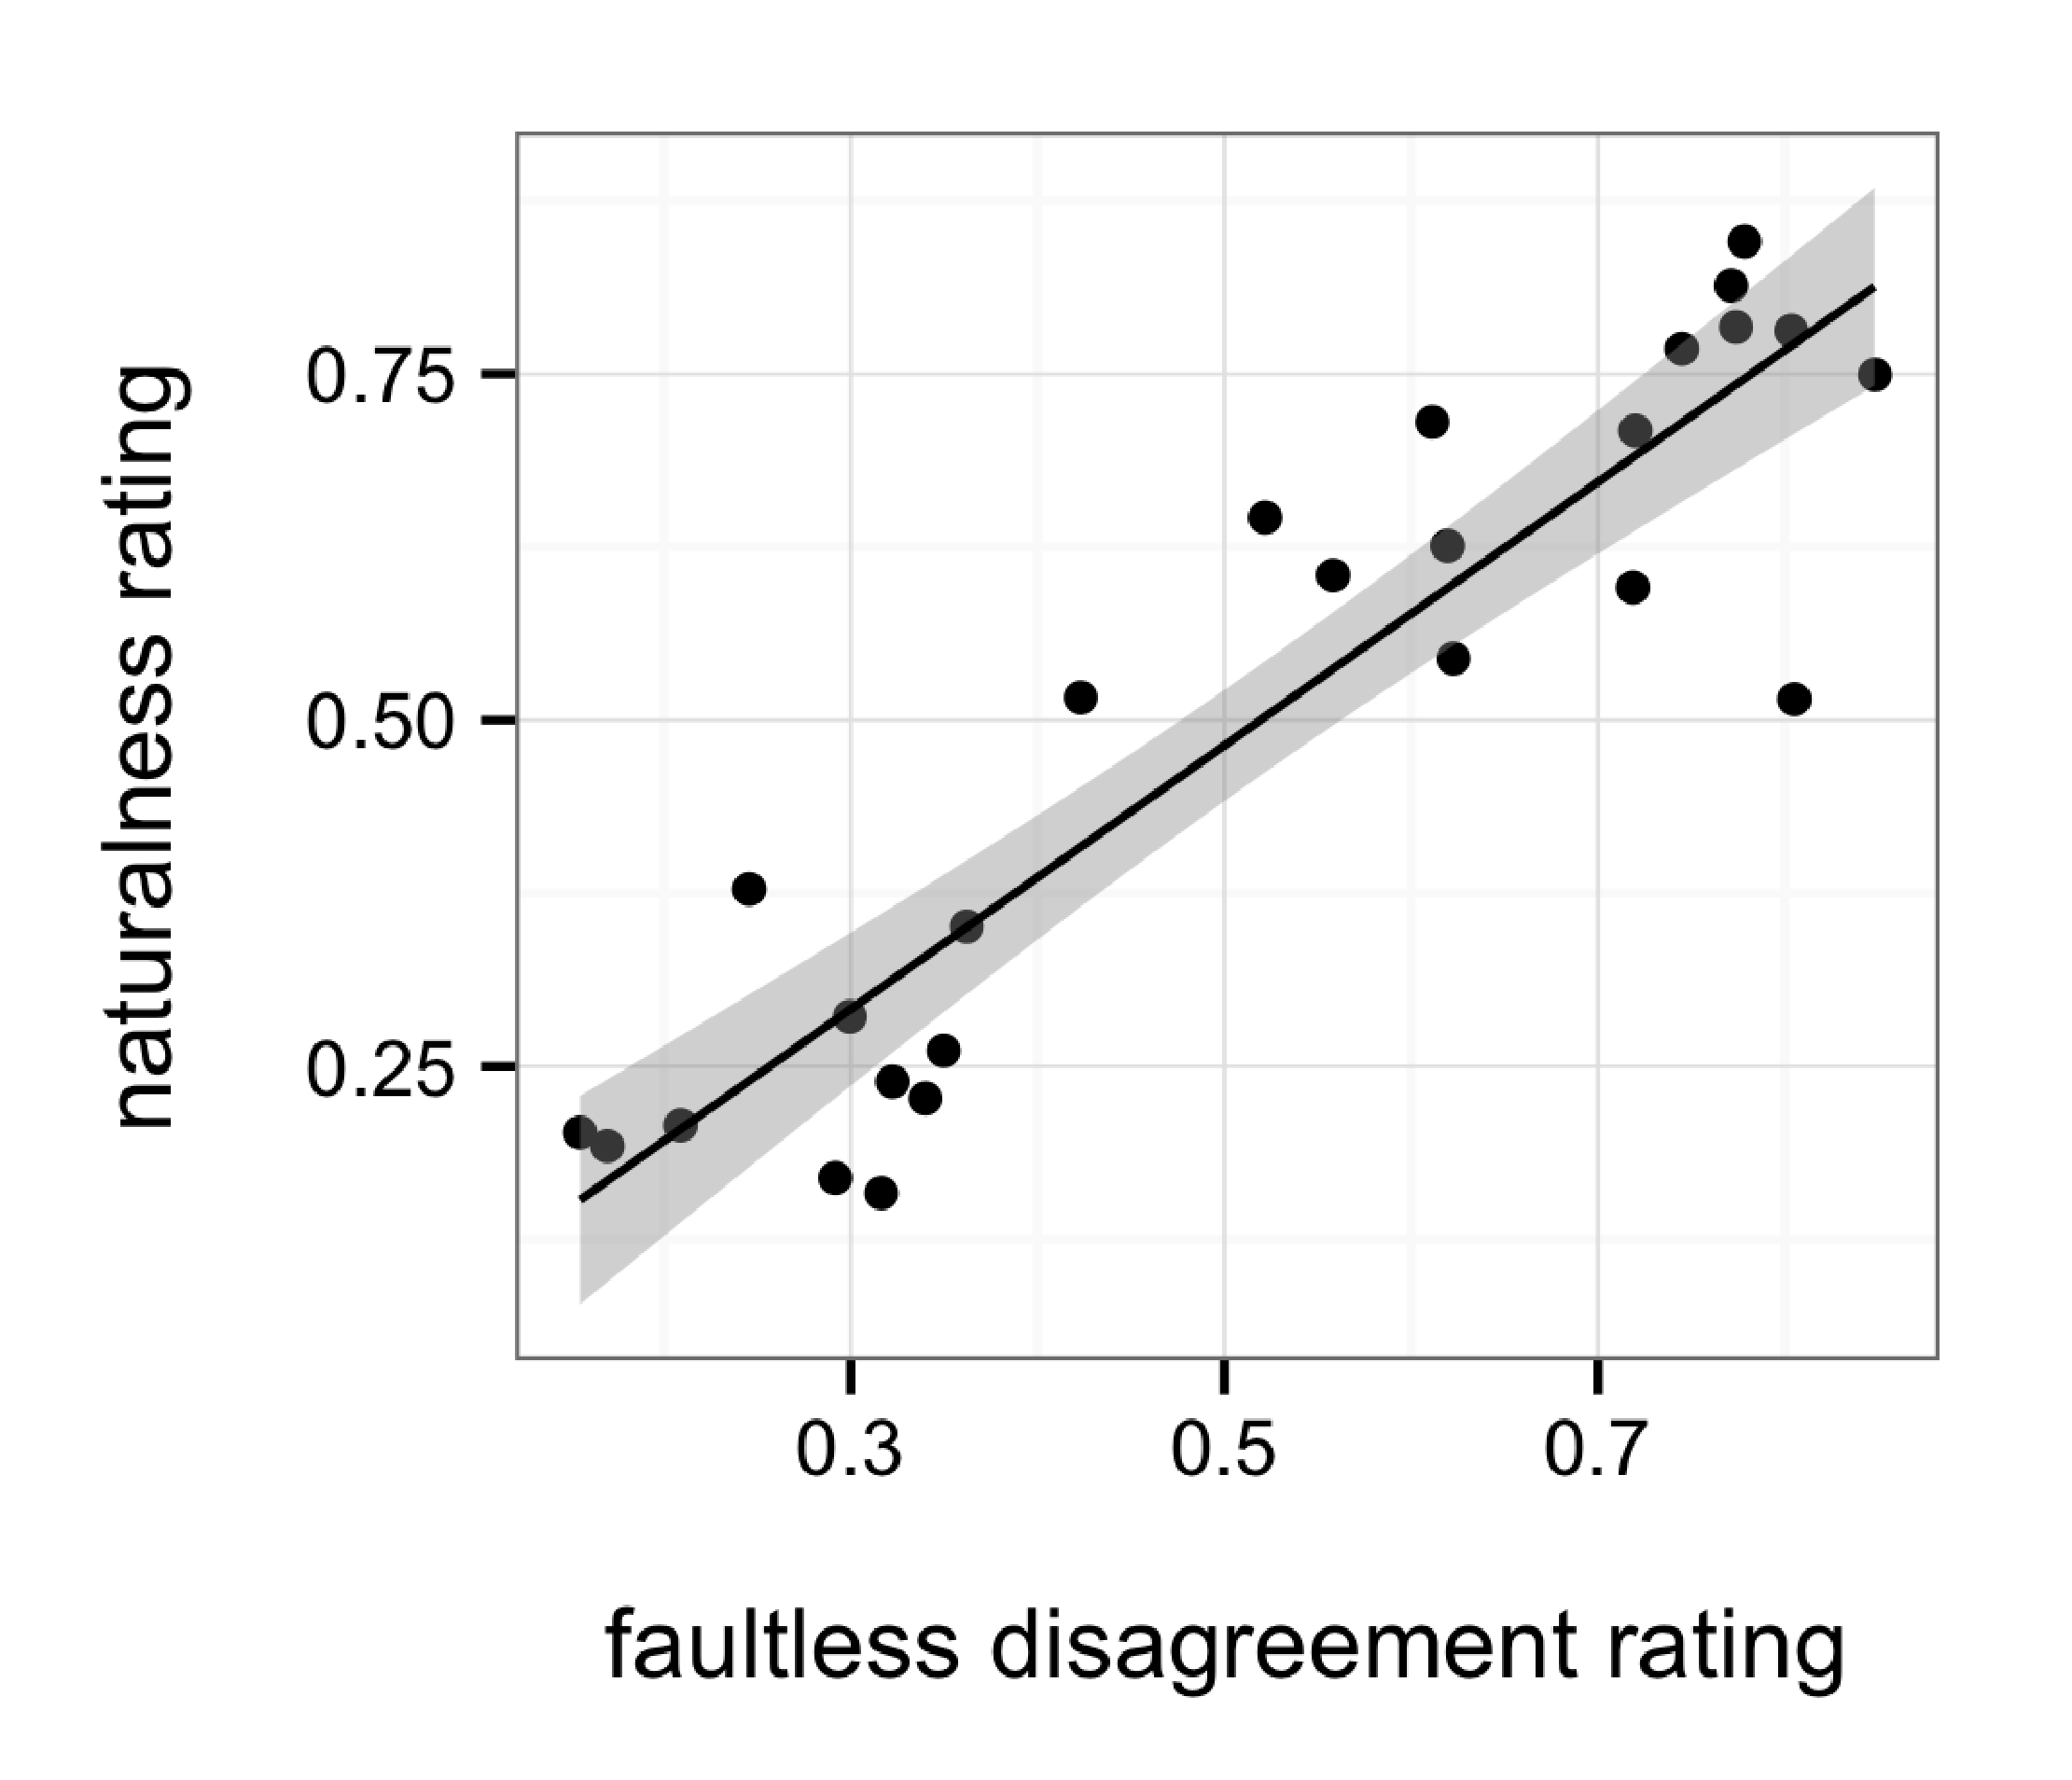
\includegraphics[width=2.8in]{plots/naturalness-faultless-new-nouns.eps}
	\caption{Mean naturalness ratings plotted against mean faultless disagreement scores for each of the 26 adjectives tested.}\label{fig:faultless}
\end{figure}



